\documentclass[tikz,border=8pt]{standalone}
\begin{document}
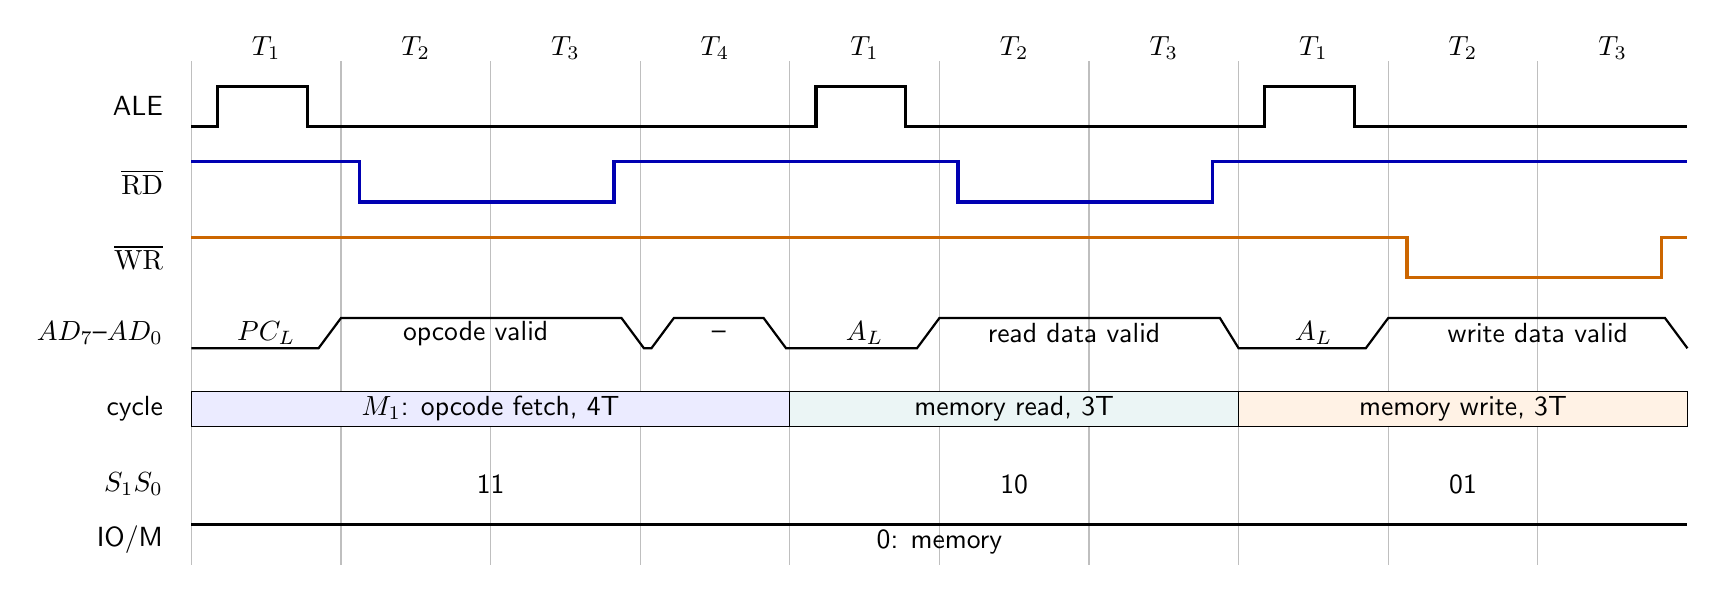
\begin{tikzpicture}[font=\sffamily,x=.95cm,y=.64cm]
\foreach \x/\t in {0/$T_1$,2/$T_2$,4/$T_3$,6/$T_4$,8/$T_1$,10/$T_2$,12/$T_3$,14/$T_1$,16/$T_2$,18/$T_3$}{\draw[gray!50] (\x,-.3)--(\x,9.7);\node at (\x+1,9.95){\t};}
\node[anchor=east] at (-.25,8.8){ALE};\node[anchor=east] at (-.25,7.3){$\overline{\rm RD}$};\node[anchor=east] at (-.25,5.8){$\overline{\rm WR}$};\node[anchor=east] at (-.25,4.3){$AD_7$--$AD_0$};\node[anchor=east] at (-.25,2.8){cycle};\node[anchor=east] at (-.25,1.3){$S_1S_0$};\node[anchor=east] at (-.25,.2){IO/M};
\draw[very thick] (0,8.4)--(.35,8.4)--(.35,9.2)--(1.55,9.2)--(1.55,8.4)--(8.35,8.4)--(8.35,9.2)--(9.55,9.2)--(9.55,8.4)--(14.35,8.4)--(14.35,9.2)--(15.55,9.2)--(15.55,8.4)--(20,8.4);
\draw[very thick,blue!70!black] (0,7.7)--(2.25,7.7)--(2.25,6.9)--(5.65,6.9)--(5.65,7.7)--(10.25,7.7)--(10.25,6.9)--(13.65,6.9)--(13.65,7.7)--(20,7.7);
\draw[very thick,orange!80!black] (0,6.2)--(16.25,6.2)--(16.25,5.4)--(19.65,5.4)--(19.65,6.2)--(20,6.2);
\draw[thick] (0,4)--(1.7,4)--(2,4.6)--(5.75,4.6)--(6.05,4)--(6.15,4)--(6.45,4.6)--(7.65,4.6)--(7.95,4)--(9.7,4)--(10,4.6)--(13.75,4.6)--(14,4)--(15.7,4)--(16,4.6)--(19.7,4.6)--(20,4);
\node at (1,4.3){$PC_L$};\node at (3.8,4.3){opcode valid};\node at (7.05,4.3){--};\node at (9,4.3){$A_L$};\node at (11.8,4.3){read data valid};\node at (15,4.3){$A_L$};\node at (18,4.3){write data valid};
\draw[fill=blue!8] (0,2.45) rectangle (8,3.15);\node at (4,2.8){$M_1$: opcode fetch, 4T};\draw[fill=teal!8] (8,2.45) rectangle (14,3.15);\node at (11,2.8){memory read, 3T};\draw[fill=orange!10] (14,2.45) rectangle (20,3.15);\node at (17,2.8){memory write, 3T};
\node at (4,1.3){11};\node at (11,1.3){10};\node at (17,1.3){01};\draw[very thick] (0,.5)--(20,.5);\node at (10,.15){0: memory};
\end{tikzpicture}
\end{document}
